% Template for ESA 6th ICATT manuscripts; to be used with:
%          spconf.sty  - LaTeX style file, and
%          IEEEbib.bst - IEEE bibliography style file.
% --------------------------------------------------------------------------
\documentclass{article}
\usepackage{spconf,amsmath,graphicx, url, listings}
\usepackage{courier, float}
\usepackage{caption}
\usepackage{subcaption}


\lstset{basicstyle=\footnotesize\ttfamily, float, language=MATLAB, breaklines=true}

% Example definitions.
% --------------------
\def\x{{\mathbf x}}
\def\L{{\cal L}}

% Title.
% ------
\title{Shape Optimisation of UAV Wing}
%
% Single address.
% ---------------
\name{Christopher Iliffe Sprague}
\address{}
%
% For example:
% ------------
%\address{School\\
%	Department\\
%	Address}
%
% Two addresses (uncomment and modify for two-address case).
% ----------------------------------------------------------
%\twoauthors
%  {A. Author-one, B. Author-two\sthanks{Thanks to XYZ agency for funding.}}
%	{School A-B\\
%	Department A-B\\
%	Address A-B}
%  {C. Author-three, D. Author-four\sthanks{The fourth author performed the work
%	while at ...}}
%	{School C-D\\
%	Department C-D\\
%	Address C-D}
%
\begin{document}

\maketitle

\begin{abstract}
    This paper examines the design of a wing for a new long-endurance aircraft that will be used as a telecommunications platform. In particular, the problem of optimizing the shape of the wing's spar, acting as the aircraft's main structural support, in order to minimize its mass, is analyzed and solved. In doing so, a robust object-orientated programming approach is taken to transcribe the problem and flexibly find optimal solutions from user defined design guesses. Using sequential quadratic programming, several numerical differentiation paradigms are investigated in relation to the problem's objective and constraints. It is shown that an optimal spar mass, over 60\% lower than the nominal, is consistently achieved while satisfying all constraints.
\end{abstract}
    
\keywords{Wing Structure, Shape Optimization}

\tableofcontents
\listoftables
\listoffigures
\lstlistoflistings

\section{Problem Model}
\subsection{Specifications}
Preceding the construction of the optimization problem, it is necessary to define the constant metrics that characterize the nature of the problem. For the case of an annular spar, the problem parametrization requires several design metrics to be taken into account, namely: wing semi-span $L$, material density $\rho$, Young's modulus $E$, ultimate tensile/compressive strength $\sigma_{max}$, aircraft operational mass $M$, minimum spar thickness $T_{min}$, minimum inner wall radius $r_{min}$, and maximum outer wall radius $R_{max}$. 

Additionally, the operational conditions that the aircraft will be subjected to need to be taken into account, namely: gravitational acceleration $g$, and maximum operational G-force $G$. In this particular investigation, attention will be directed towards the case of a carbon fiber spar, whose specifications are enumerated in Table \ref{specs}. One can instantiate a UAV of this nature through an object-oriented approach, as shown in Listing \ref{UAV}. The full source code of the UAV class is shown in Listing \ref{uavclass}.

\begin{lstlisting}[caption=UAV Instantiation, label=UAV, float]
% Instantiate the UAV
Raptor = UAV(... % With properties:
  7.5,       ... % Wing semi-span [m].
  1600,      ... % Spar density [kg/m^3].
  7e10,      ... % Modulus of elasticity [Pa].
  600e6,     ... % Maximum spar strength [Pa].
  500,       ... % Mass of aircraft [Kg].
  9.807,     ... % Earth's gravity [m/s^2].
  2.5e-3,    ... % Minimum spar thickness [m].
  1e-2,      ... % Minimum inner spar radius [m].
  5e-2,      ... % Maximum outer spar radius [m].
  2.5        ... % Maximum operational G-force.
  );
\end{lstlisting}

\begin{table}
\centering
\caption{Problem Specifications}
\begin{tabular}{|l|l|l|}
\hline
Parameter            & Symbol    & Value         \\ \hline
Semi-Span            & $L$       & $7.5~m$       \\ \hline
Density              & $\rho$    & $1600~kg/m^3$ \\ \hline
Young's Modulus      & $E$       & $70~GPa$      \\ \hline
Ultimate Strength             & $\sigma_{max}$  & $600~MPa$     \\ \hline
Aircraft Mass                 & $M$       & $500~kg$      \\ \hline
Minimum Thickness    & $T_{min}$ & $2.5~mm$      \\ \hline
Minimum Inner Radius & $r_{min}$ & $1~cm$        \\ \hline
Maximum Outer Radius & $R_{max}$ & $5~cm$        \\ \hline
Gravity              & $g$       & $9.81~m/s^2$  \\ \hline
G-Force              & $G$       & $2.5$         \\ \hline
\end{tabular}
\label{specs}
\end{table}

\subsection{Problem Formulation}\label{opt}
The objective of this optimization problem is to minimize the total mass of the spar while not allowing its structural stress $\sigma$ at any spanwise location to exceed its material's ultimate strength $\sigma_{max}$ during its maximal operational loading conditions. Additionally, there are also manufacturing constraints that dictate the spar's inner radius $r$ and outer radius $R$ to satisfy $r \geq r_{min}$ and $R \leq R_{max}$, while satisfying a thickness constraints $R - r \geq T_{min}$. In a more formal manner, this problem's formulation is shown as follow:
$$
\begin{aligned}
& \underset{\mathbf{R}}{\text{minimize}} 
& & m(\mathbf{R}) \mid \mathbf{R} \mapsto \{ r(x), R(x) \} \mid x \in [0,L] \\
& \underset{\forall x}{\text{subject to}}
& &  r_{min} \leq r(x) \leq r_{min} + T_{min}\\
& & & R_{max} - T_{min} \leq R(x) \leq R_{max}\\
& & & r(x) - R(x) \leq -T_{min} \\
& & & \sigma(x) - \sigma_{max} \leq 0
\end{aligned}
$$
Essentially, the annular spar's inner and outer spanwise radii $\{ r(x), R(x) \}$ must be manipulated until the spar's total mass $m(\mathbf{R})$ has reached a minimum value for all possible satisfactory forms of $r(x)$ and $R(x)$. 

\subsection{Geometrical Parametrization}
Because finite element methods will be used to solve this optimization problem, it is required to discretize the spar's geometry into a series of spanwise finite elements. Herein, the wing's spar will be represented by a series of nodes, indexed by $i$, where $i=1$ and $i=n$ signify the locations of the wing's root and tip respectively. As such, it can be deduced that there are $n$ nodes and $n-1$ finite elements along the span of the spar. Hence, the set of node indexes $\mathcal{N}$ and finite element indexes $\mathcal{E}$ are defined as follows
$$
\begin{gathered}
\mathcal{N} = [i, i+1, \dots, n] \\
\mathcal{E} = [j, j+1, \dots, n-1]
\end{gathered}
$$


\subsubsection{Design Vector}\label{R}
It is appropriate to begin the optimization process with the formulation of the design vector $\mathbf{R}$, composed of inner radii $r$ and outer radii $R$. Abiding to the form of a column vector, it is necessary to apply a change of variables and define the design vector as follows,
$$
\begin{gathered}
\mathbf{R} = [\xi_k, \xi_{k+1}, \dots, \xi_{2n}]^T \\
\{\xi_{2k-1}, \xi_{2k}\} \leftarrow \{r_i, R_i\} \forall i \in \mathcal{I}
\end{gathered}
$$
It can be seen that the inner and outer radii are sequenced to occur for every other index in the design vector $\mathbf{R}$.

\subsubsection{Spanwise Location}
Having deduced the number of nodes $n$ from the user supplied design vector, the spanwise location along the spar can be discretized in a similar manner as, $$ \mathbf{x} = [ x_i, x_{i+1}, \dots, x_n] \mid x_1 = 0 , x_n = L$$, where it is noted that the first and final index values of $x_i$ satisfy the length of the wing's semi-span.

\subsubsection{Volume and Mass}
At each node $i$ along the wing's span, the spar's cross section is represented as a circular annulus of inner and outer radii, $r_i$ and $R_i$, respectively, whose area is defined by $ A_i = \pi (R_i^2 - r_i^2) $. Assuming this cross sectional area characterization is consistent across all nodes, the inner and outer surfaces of each finite element $j$ are linearly interpolated between their corresponding nodes $i=j$ and $i=j+1$. Hence the nodes' cross sectional areas are integrated along the interpolations, yielding the volume of each finite element as follows
$$V_j = \frac{\pi}{3} (r_j^2 - R_j^2 + r_j r_{j+1} - R_j R_{j+1} + r_{j+1}^2 - R_{j+1}^2 )(x_j - x_{j+1}) $$ 
As such, the total volume of the spar can be computed by a summation across all finite elements $V=\sum_{j=1}^{n-1} V_j$. Subsequently the spar's total mass is obtained as $m=\rho V$, and hence the optimization problem's objective function $m(\mathbf{R})$.

\subsection{Material Stress Constraints}
As formulated in Section \ref{opt}, the structural stress at any spanwise location along the spar must not exceed its material's ultimate strength, $\sigma_i - \sigma_{max} \leq 0 ~ \forall i \in \mathcal{I}$. Modeling the wing's spar as a cantilever beam, Euler-Bernoulli beam theory can be exploited to compute the spar's nodal stress.

\subsubsection{Load Distribution}
In this study, it is assumed that the force distribution in the spanwise direction has an approximately linear distribution, with maximum load at the root and zero load at the tip. Hence the force at each node can be formulated as follows
$$ F_i = \frac{GMg}{L} \left ( 1-\frac{x_i}{L} \right )$$ With the specifications given in Table \ref{specs} and Listing \ref{UAV}, the nature of the spar's force distribution can be seen in Figure \ref{fig:force}.

\begin{figure}
    \caption{Spanwise Force Distribution.}
    \centering
    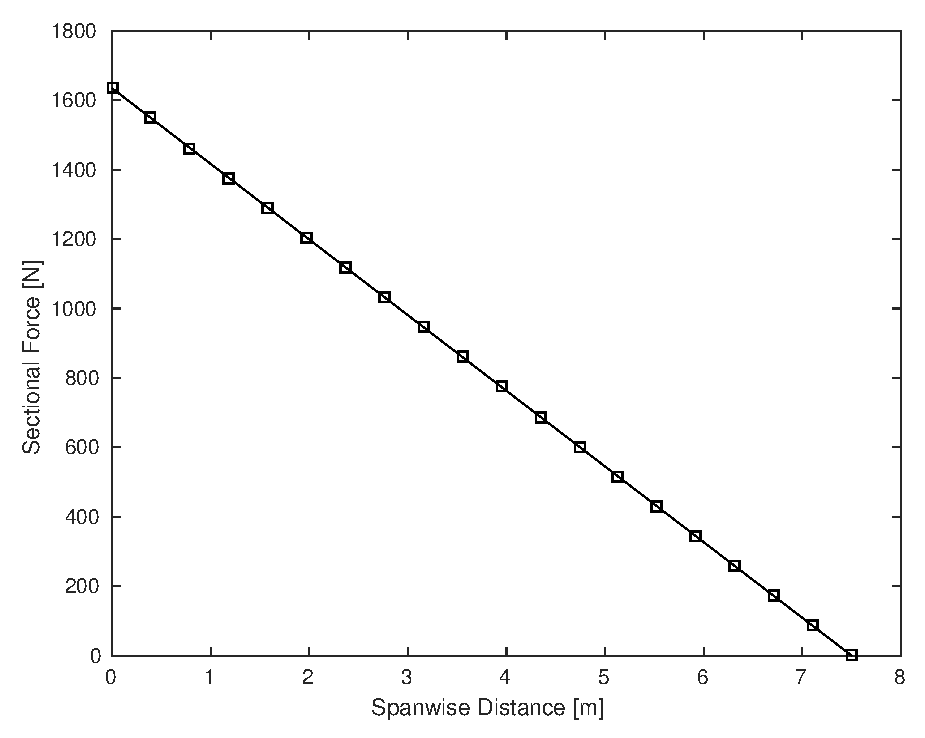
\includegraphics[width=0.48\textwidth]{Pics/Span_Force.eps}
    \label{fig:force}
\end{figure}

\subsubsection{Second Moment of Area}
In order to calculate the displacement of the spar at any location along its span, the second moment of inertia at each node must first be calculated. For a circular annulus describing the cross section of any node along the spar's span, the second moment of area is formulated as such
$$ I_i = \frac{\pi}{4} \left ( R_i^4 - r_i^4 \right )$$

\subsubsection{Displacement and Stress}
Assuming a transversely applied load distribution and cross sectional symmetry, a cubic Hermite finite-element basis is used to solve the Euler-Bernoulli beam equations. The vertical and angular displacement of the spar at each node along the beam are calculated, using the aforementioned formulations of the load distribution and second moment of area. The beam's vertical displacement is formulated as follows $ \mathbf{\delta} = [\delta_i, \delta_{i+1}, \dots, \delta_n]^T $. Using the spar's displacements, its nodal tensile stresses are computed and formulated as such
$\mathbf{\sigma} = [\sigma_i, \sigma_{i+1}, \dots, \sigma_n]^T $. Hence the constraint function must satisfy the following 
$$\sigma_i - \sigma_{max} \leq 0 ~\forall i \in \mathcal{I}$$ 
Because the derivation of this method is beyond the scope of this paper, the reader is advised to consult \cite{Kuo2006} for further information.

\subsection{Manufacturing Constraints}
As required by the optimization problem's specifications, the inner and outer radii of each annular cross section cannot be less than $T_{min}$ apart, the inner radius cannot be smaller than $r_{min}$, and the outer radius cannot be larger than $R_{max}$.

\subsubsection{Radii Bounds}
In formulating the range to which the inner radii $r_i$ and outer radii $R_i$ are bounded, it is necessary to formally define lower and upper bound vectors $\mathbf{L}$ and $\mathbf{U}$, respectively, that satisfy $\mathbf{L} \leq \mathbf{R} \leq \mathbf{U}$, corresponding to the form of the transformed design vector $\mathbf{R}$ described in Section \ref{R}. The lower and upper bounds for the radii, corresponding to the constraints described in Section \ref{opt}, are formulated as such
$$
\begin{gathered}
\mathbf{L} = [\lambda_k, \dots, \lambda_{2n}]^T \mid \{ \lambda_{2k-1}, \lambda_{2k} \} \leftarrow \{ r_{min}, r_{min} + T_{min} \} \\
\mathbf{U} = [\upsilon_k, \dots, \upsilon_{2n}]^T \mid \{ \upsilon_{2k-1}, \upsilon_{2k} \} \leftarrow \{ R_{max} - T_{min}, R_{max} \}
\end{gathered}
$$

\subsubsection{Thickness}
In order to enforce the constraint that the annular spar's wall thickness may not be smaller than $T_{min}$ and that the outer radii must always be greater than the inner radii $R_i > r_i ~ \forall i \in \mathcal{I}$, linear inequality constraints must be instantiated. In doing so, it is required to formulate a $n \times 2n$ matrix $\mathbf{A}$ and $n \times 1$ column vector $\mathbf{b}$ that satisfy $\mathbf{A}\mathbf{R} \leq \mathbf{b}$. The matrices are defined as follows
$$
\begin{gathered}
\mathbf{A} = 
 \begin{bmatrix}
  \alpha_{i,k} & \cdots & \alpha_{i,2n} \\
  \vdots  & \ddots & \vdots  \\
  \alpha_{n,k} & \cdots & \alpha_{n,2n} \\
 \end{bmatrix}
 \mid \{ \alpha_{i,2i-1}, \alpha_{i,2i} \} \leftarrow \{1,-1 \} \\
 \mathbf{b} = [\beta_i, \dots, \beta_n]^T \mid \beta_i \leftarrow -T_{min}
\end{gathered}
$$
where $\mathbf{R}$ is defined as the $2n \times 1$ column vector described in Section \ref{R}. For further information on formatting constraints and objectives to accommodate Matlab's built in functions, the reader is advised to consult \cite{Attaway2013}.

\section{Optimization}
\subsection{Sequential Quadratic Programming}
Sequential quadratic programming (SQP) has proven itself as one of the most successful methods for solving nonlinearly constrained optimization problems. Essentially, SQP aims to model the nonlinear programming problem (NLP) at a given approximate solution $\mathbf{R}^h$ by a quadratic programming subproblem, then use the subproblem to construct a better approximation $\mathbf{R}^{h+1}$. This process is iterated until convergence to a solution $\mathbf{R}^*$ is achieved. SQP is not a feasible point method; neither the point nor any of the subsequent iterates are required to be feasible. However, the SQP method does satisfy the bounds $\mathbf{L}$ and $\mathbf{U}$ at every iteration, and is ideal for small to medium scale problem such as in the case of this paper's optimization problem, where optimality returns are generally diminished for $n>40$. This method of nonlinear constrained optimization is handled natively by Matlab's \lstinline{fmincon} function \cite{Attaway2013}, and described in more detail in \cite{Boggs1995}.

\subsection{Objective and Constraint Gradients}
In order to achieve an optimal design vector $\mathbf{R}^*$ that satisfies $m(\mathbf{R}^*) \leq m(\mathbf{R}) \forall \mathbf{R} \mapsto \{r_i, R_i\} \forall i \in \mathcal{I}$, both the necessary and sufficient conditions for optimality need to be realized. It is necessary for an optima at a stationary point $\mathbf{\bar{R}}$ to have a first derivative of zero $\nabla \mathbf{\bar{R}} = \mathbf{0}$. It is sufficient to call the stationary point a local minimum $\mathbf{R^*}$ if $\nabla^2 \mathbf{R^*} > \mathbf{0}$. For further information on conditions of optimality, the reader should consult \cite{Kuhn1951}.

\subsubsection{Forward Difference}
Among the simplest methods of finite difference derivative approximations is the forward step method
$$ \mathbf{\nabla}_{\xi_i}\mathbf{f}(\mathbf{R}) =
\frac{\mathbf{f}(\mathbf{R} + h_i\mathbf{e}_i) - \mathbf{f}(\mathbf{R})}{h_i} + \mathcal{O}(h_i)$$
, where $\mathbf{e}_i$ represents a vector of zeros with the $i^{th}$ index equal to $1$, $\mathcal{O}(h_i)$ represents the truncation error, and $h_i$ represents the step size. Herein, $h_i$ represents the positive distance from $\lvert \xi_i \rvert$ to the next larger floating-point number of the same precision as $\xi_i$. It should be noted that $\mathbf{f}$ may represent either the problem's objective function $m(\mathbf{R})$ or constraint function $\mathbf{c}(\mathbf{R})$.

\subsubsection{Central Difference}
Similarly to the forward difference method, the approximate derivative of either the objective or constraint functions may be approximated with a perturbation to the design vector $\mathbf{R}$. Under the central difference paradigm, the finite difference derivative approximation becomes
$$ \mathbf{\nabla}_{\xi_i}\mathbf{f}(\mathbf{R}) =
\frac{\mathbf{f}(\mathbf{R} + h_i\mathbf{e}_i) - \mathbf{f}(\mathbf{R} - h_i\mathbf{e}_i)}{2h_i} + \mathcal{O}(h_i^2)$$
It should be noticed that the central difference method is second-order accurate since the dominate term in its truncation error is $\mathcal{O}(h_i^2)$. Therefor the central difference method is more accurate than the forward difference method due to its smaller truncation error.

\subsubsection{Complex Step}
Among the best of the finite difference methods is complex-step. It has shown to be very accurate, robust, and easy to implement, while maintaining a reasonable computational cost. The relationship between the real and imaginary parts of the function at hand is exploited to yield a derivative approximation of the following form
$$ \mathbf{\nabla}_{\xi_i}\mathbf{f}(\mathbf{R}) =
\frac{\Im [ \mathbf{f}(\mathbf{R} + h_i\mathbf{e}_i \sqrt{-1}) ] }{h_i} + \mathcal{O}(h_i^2)$$

The complex step method converges quadratically with decreasing step size. This method is particularly advantageous because it is insensitive to small step sizes and eventually achieves the accuracy of its function evaluations. The reader can learn more about its derivation in \cite{Lyness1968}. Herein, focus will be directed towards the use of the complex step method to approximate the gradients of both the objective function $m(\mathbf{R})$ and constraint function $\mathbf{C}(\mathbf{R})$. The complex step method can be formulated to approximate the functions' Jacobian matrices as shown in Listing \ref{complexalg}. As an example, to approximate the gradient of the objective function, one should execute \lstinline[breaklines=true]{obj.Complex_Jacobian(@obj.Stress_Constraints, R)}.

\begin{lstlisting}[caption=Complex Step Method, label=complexalg, float]
function jac = Complex_Jacobian(obj, funct, R)
  fval = funct(R);
  n    = numel(R);
  m    = numel(fval);
  jac  = zeros(m,n);
  h    = eps(R)*n;
  for I=1:n
    r        = R;
    r(I,1)   = r(I,1) + h(I,1)*i;
    jac(:,I) = imag(funct(r))/h(I,1);
  end
  jac = jac.';
end
\end{lstlisting}

\section{Results}
Having instantiated an aircraft with the specifications enumerated in Table \ref{specs}, one can supply an initial guess to the optimizer. For the sake of testing robustness, the initial guess of the $2n \times 1$ design vector $\mathbf{R_0}$ will characterize the boundary constraints of the spar's radii, such that $ \{r_i, R_i\} \leftarrow \{r_{min}, R_{max} \} \forall i \in \mathcal{I}$, yielding an initial total spar mass of $m_0 = 90.4779~kg$, far beyond the desired optimal value $m^* < 5~kg$.

One can easily instantiate an initial guess $\mathbf{R_0}$ of the design vector, with $n=20$ nodes for instance, as shown in Listing \ref{40n}. 
\begin{lstlisting}[caption=20 Node Design Vector, label=40n]
% Take an initial guess of the spar's radii.
R = zeros(40,1);
for I=1:Raptor.N_Nodes(R)
    R(2*I-1,1) = Raptor.Rimin;
    R(2*I, 1)  = Raptor.Romax;
end
\end{lstlisting}
Once the design vector has been characterized, the user can easily begin the optimization process by executing \lstinline[breaklines=true]{[Ropt,fval,exitflag,output,lambda,grad,hessian] = Raptor.Optimize(R, step_type);}, where \lstinline{step_type} can be \lstinline{'forward'}, \lstinline{'central'}, or \lstinline{'complex'}. With $n=20$ nodes, the forward, central, and complex step optimization processes yield the outputs in Listings \ref{forward40}, \ref{central40}, and \ref{complex40}, respectively. It can quite easily be seen that all three of the finite difference methods yield approximately equal values of the optimal spar mass $m^* = 4.9069$, thereby verifying beyond a doubt that $m^*$ is certainly a local minimum of the optimization problem. 

Visually, the spar geometry, vertical displacement, and stress can be see for all the finite difference methods in Figures \ref{fig:forward40}, \ref{fig:central40}, and \ref{fig:complex40}. Additionally, the iterative convergence of the objective function can be see for each method in Figure \ref{fig:opt40}. It can be seen that each finite difference method yields virtually identical results. Each method yielded a final spar mass that is $63\%$ better than the nominal mass of $13.26~kg$. However, it was quite apparent that the optimization process using the complex step method was far more expeditious than the other methods.

\section{Conclusions}
A virtually identical value of the spar's optimal mass $m^* = 4.9069$, over $60\%$ better than the nominal mass, has been achieved consistently across three separate finite difference methods. Validity can thereby be concluded for the optimality of the resultant masses and design vectors, as well as the method by which the complex Jacobian matrices were computed in the complex step implementation. Through implementation, as expected, it was seen that the complex step method yielded solution convergence in a fraction of the time it took the forward and central step methods to do so. Lastly, from the geometrical representations of the resulting design vectors, an intuition can be developed, from which a wing's spar will tend to have greater radii towards its root. It can be seen that the optimization process has indeed solidified this intuition, by yielding geometries which meet the upper constraints towards the root and lower constraints towards the tip.

\bibliography{refs.bib} 
\bibliographystyle{IEEEtran}

\section{Appendix}
\subsection{Optimization Outputs}
\begin{lstlisting}[caption=Forward Step Output, label=forward40, float]
fval =

    4.9069


output = 

         iterations: 19
          funcCount: 848
          algorithm: 'sqp'
            message: 'Local minimum found that satisfies the constraints.…'
    constrviolation: 4.7705e-18
           stepsize: 1.2194e-14
       lssteplength: 1
      firstorderopt: 9.1052e-14
\end{lstlisting}

\begin{lstlisting}[caption=Central Step Output, label=central40, float]
fval =

    4.9069


output = 

         iterations: 19
          funcCount: 848
          algorithm: 'sqp'
            message: 'Local minimum found that satisfies the constraints.…'
    constrviolation: 4.7705e-18
           stepsize: 1.2194e-14
       lssteplength: 1
      firstorderopt: 9.1052e-14
\end{lstlisting}

\begin{lstlisting}[caption=Complex Step Output, label=complex40, float]
fval =

    4.9069


output = 

         iterations: 17
          funcCount: 43
          algorithm: 'sqp'
            message: 'Local minimum found that satisfies the constraints.…'
    constrviolation: 4.7705e-18
           stepsize: 1.8812e-14
       lssteplength: 0.7000
      firstorderopt: 8.7522e-14

\end{lstlisting}

\subsection{Optimization Figures}
\begin{figure}[H]
    \centering
    \caption{Forward Difference with 20 Nodes}
    \label{fig:forward40}
    \begin{subfigure}[b]{0.5\textwidth}
        \caption{Geometry}
        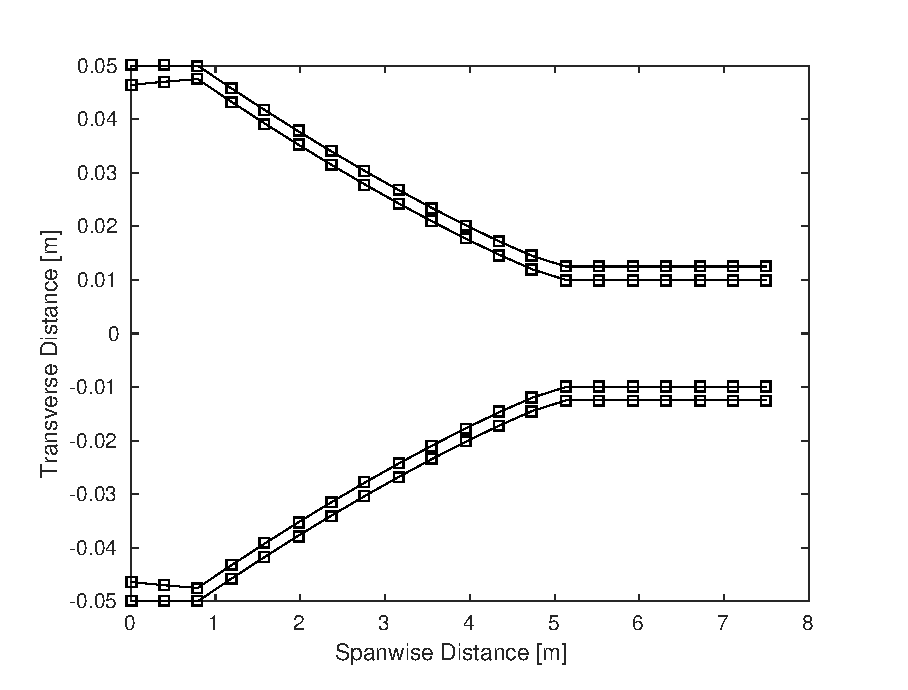
\includegraphics[width=\textwidth]{Pics/forward40shape.eps}
        
    \end{subfigure}
    ~ %add desired spacing between images, e. g. ~, \quad, \qquad, \hfill etc. 
      %(or a blank line to force the subfigure onto a new line)
    \begin{subfigure}[b]{0.5\textwidth}
        \caption{Vertical Displacement}
        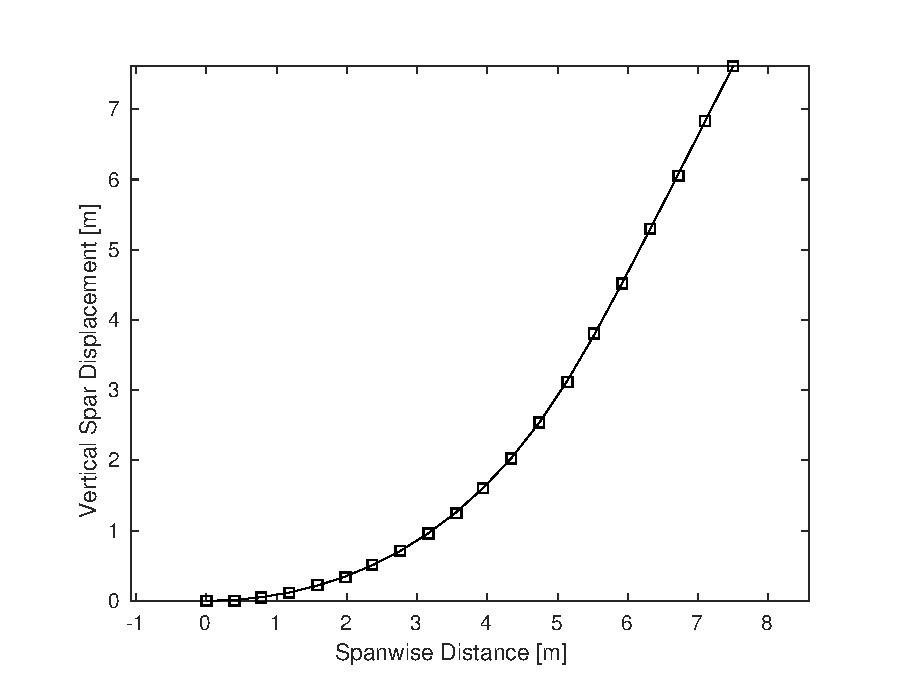
\includegraphics[width=\textwidth]{Pics/forward40disp.eps}
        
    \end{subfigure}
    ~ %add desired spacing between images, e. g. ~, \quad, \qquad, \hfill etc. 
    %(or a blank line to force the subfigure onto a new line)
    \begin{subfigure}[b]{0.5\textwidth}
        \caption{Stress}
        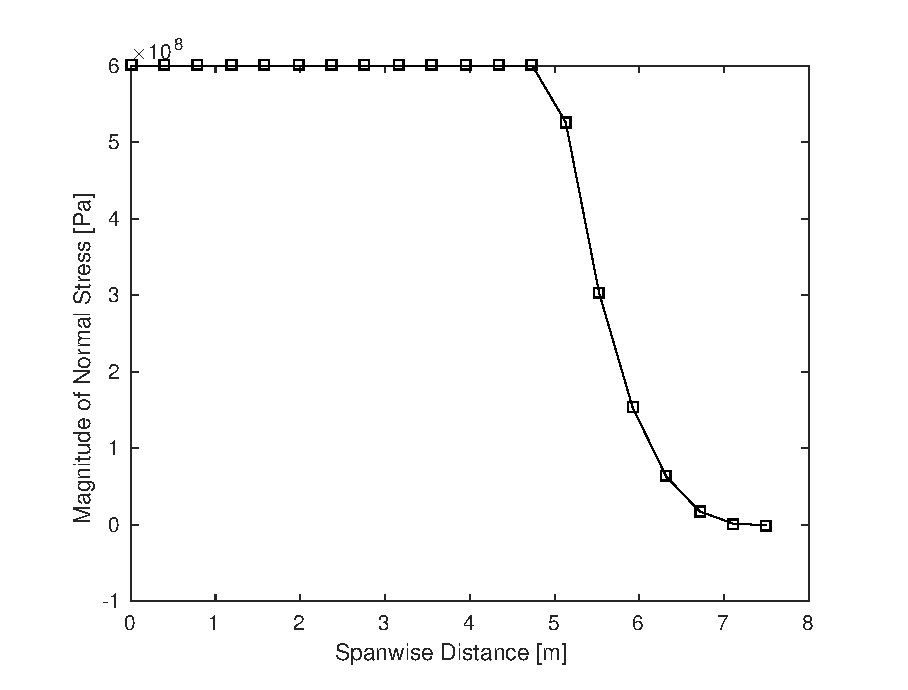
\includegraphics[width=\textwidth]{Pics/forward40stress.eps}
        
    \end{subfigure}
\end{figure}

\begin{figure}[H]
    \centering
    \caption{Central Difference with 20 Nodes}
    \label{fig:central40}
    \begin{subfigure}[b]{0.5\textwidth}
        \caption{Geometry}
        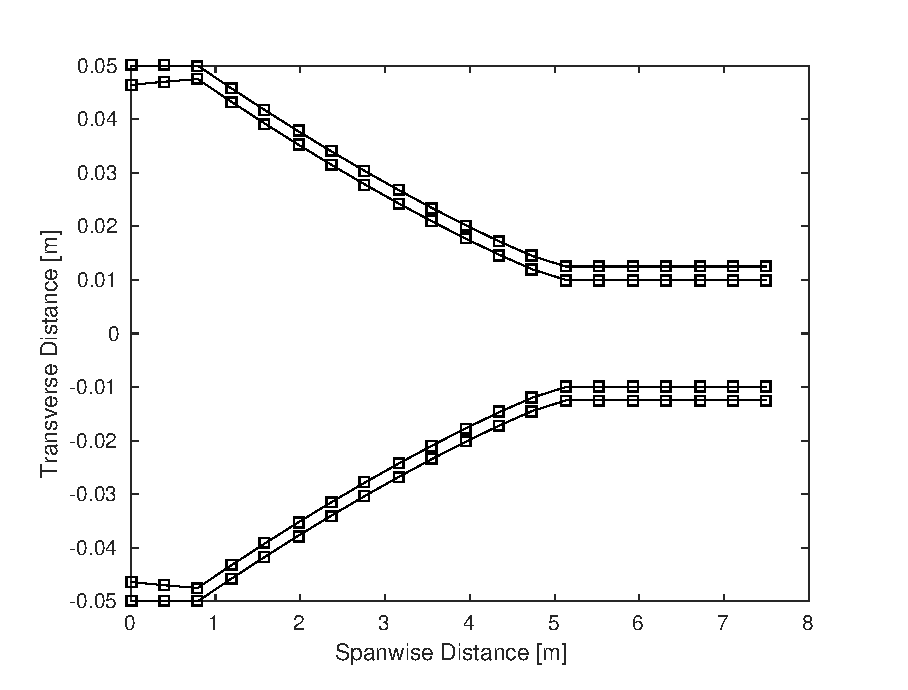
\includegraphics[width=\textwidth]{Pics/central40shape.eps}
        
    \end{subfigure}
    ~ %add desired spacing between images, e. g. ~, \quad, \qquad, \hfill etc. 
      %(or a blank line to force the subfigure onto a new line)
    \begin{subfigure}[b]{0.5\textwidth}
        \caption{Vertical Displacement}
        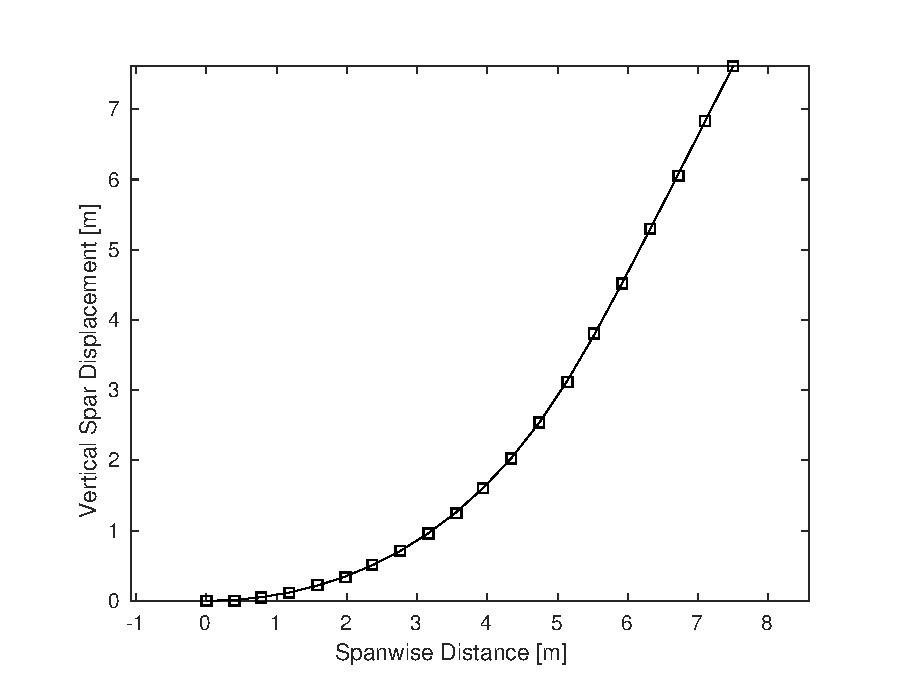
\includegraphics[width=\textwidth]{Pics/central40disp.eps}
        
    \end{subfigure}
    ~ %add desired spacing between images, e. g. ~, \quad, \qquad, \hfill etc. 
    %(or a blank line to force the subfigure onto a new line)
    \begin{subfigure}[b]{0.5\textwidth}
        \caption{Stress}
        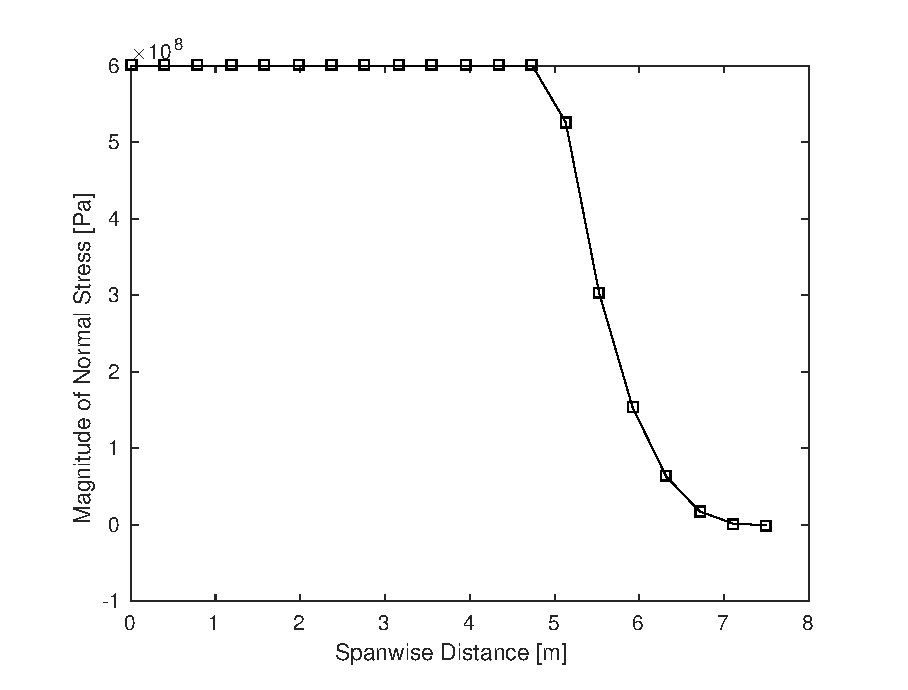
\includegraphics[width=\textwidth]{Pics/central40stress.eps}
        
    \end{subfigure}
\end{figure}

\begin{figure}[H]
    \centering
    \caption{Complex Difference with 20 Nodes}
        \label{fig:complex40}
    \begin{subfigure}[b]{0.5\textwidth}
        \caption{Geometry}
        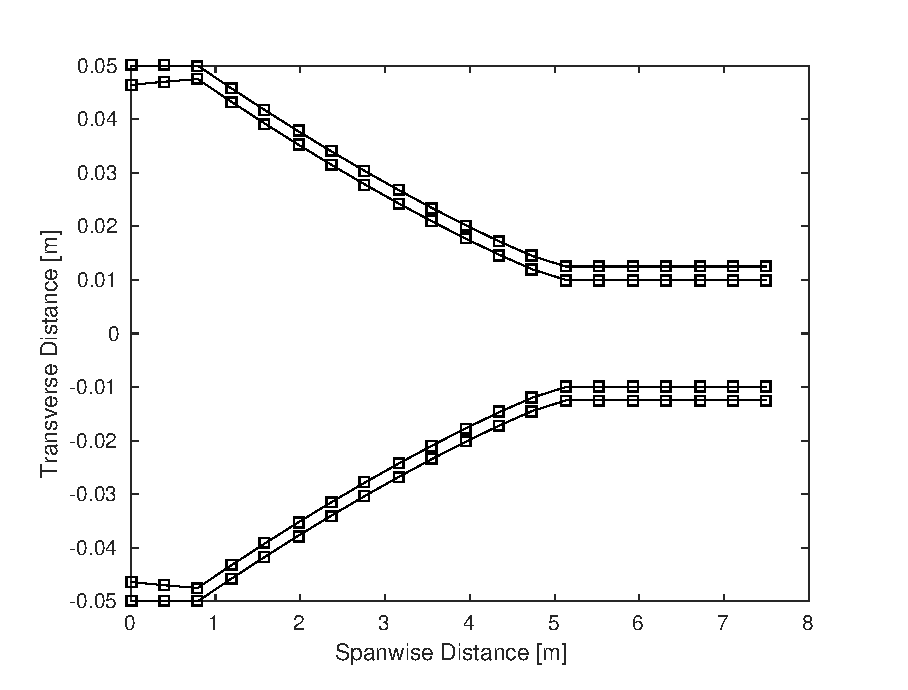
\includegraphics[width=\textwidth]{Pics/complex40shape.eps}
        
    \end{subfigure}
    ~ %add desired spacing between images, e. g. ~, \quad, \qquad, \hfill etc. 
      %(or a blank line to force the subfigure onto a new line)
    \begin{subfigure}[b]{0.5\textwidth}
        \caption{Vertical Displacement}
        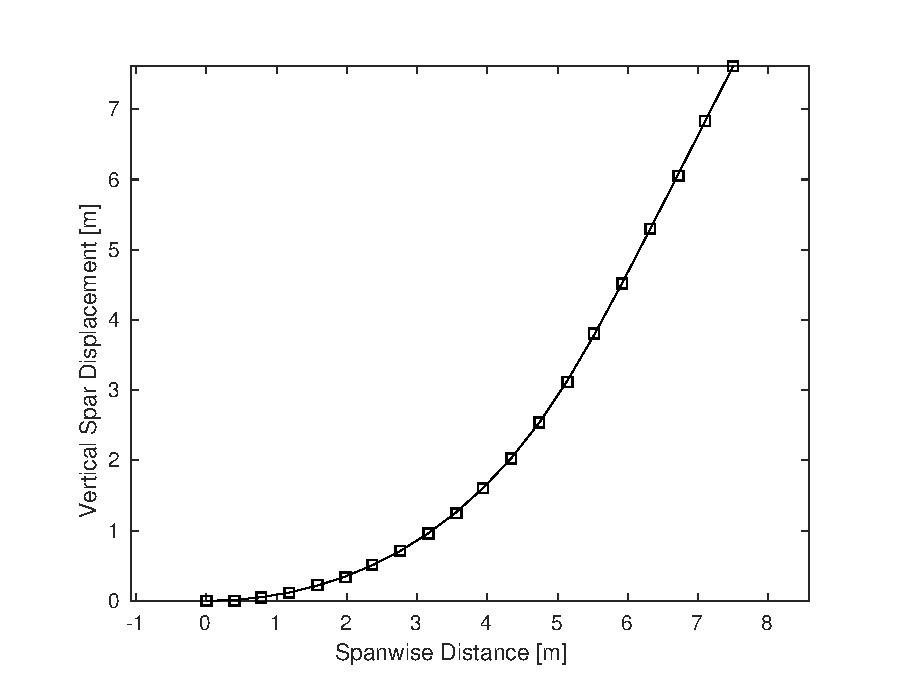
\includegraphics[width=\textwidth]{Pics/complex40disp.eps}
        
    \end{subfigure}
    ~ %add desired spacing between images, e. g. ~, \quad, \qquad, \hfill etc. 
    %(or a blank line to force the subfigure onto a new line)
    \begin{subfigure}[b]{0.5\textwidth}
        \caption{Stress}
        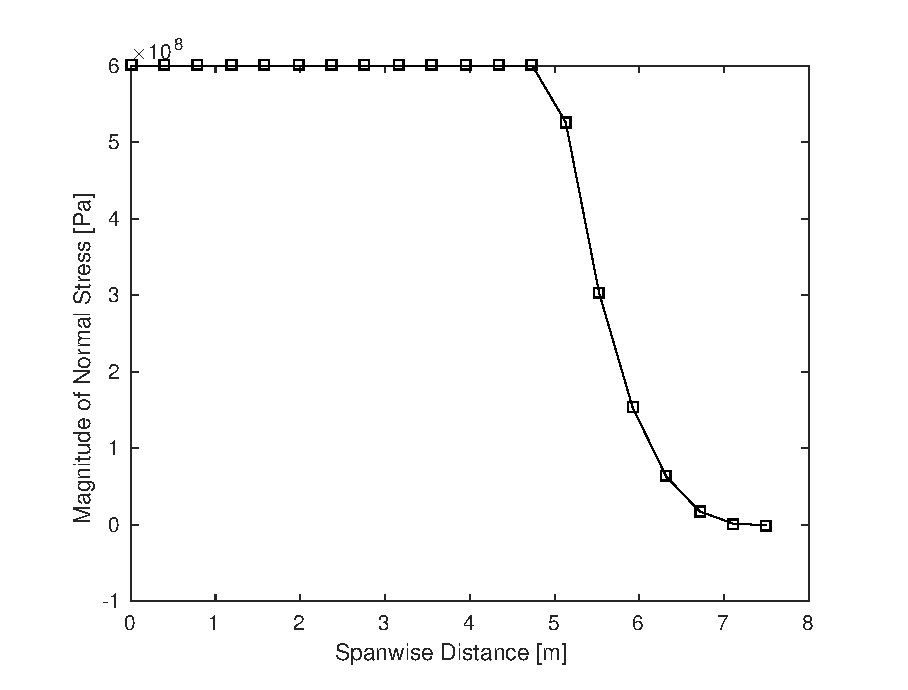
\includegraphics[width=\textwidth]{Pics/complex40stress.eps}
        
    \end{subfigure}
\end{figure}

\begin{figure}[H]
    \centering
    \caption{Objective Convergence with 20 Nodes}
        \label{fig:opt40}

    \begin{subfigure}[b]{0.45\textwidth}
        \caption{Forward Difference}
        \includegraphics[width=\textwidth]{Pics/forward40opt.eps}
        
    \end{subfigure}
    ~ %add desired spacing between images, e. g. ~, \quad, \qquad, \hfill etc. 
      %(or a blank line to force the subfigure onto a new line)
    \begin{subfigure}[b]{0.45\textwidth}
        \caption{Central Difference}
        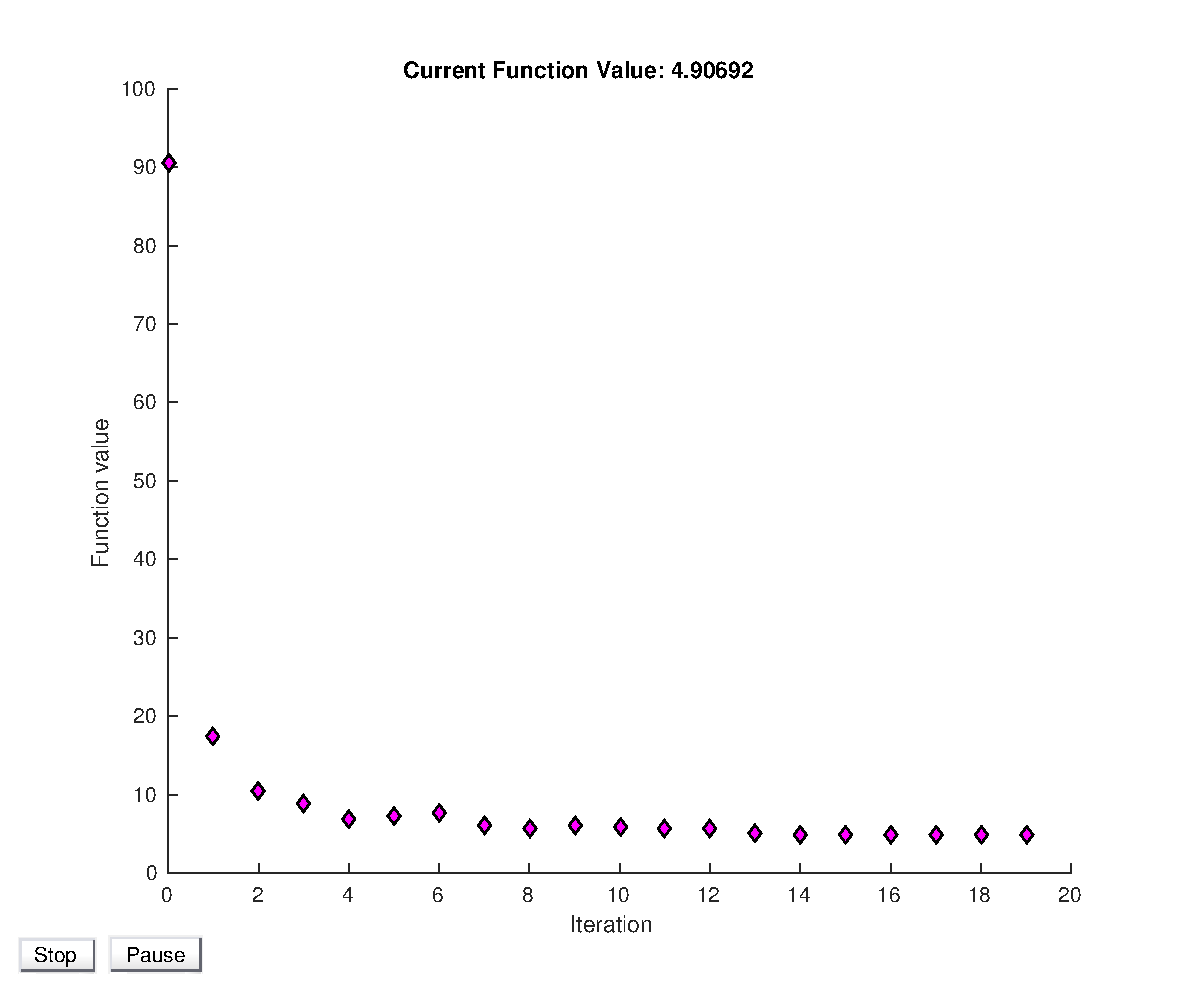
\includegraphics[width=\textwidth]{Pics/central40opt.eps}
        
    \end{subfigure}
    ~ %add desired spacing between images, e. g. ~, \quad, \qquad, \hfill etc. 
    %(or a blank line to force the subfigure onto a new line)
    \begin{subfigure}[b]{0.45\textwidth}
        \caption{Complex Difference}
        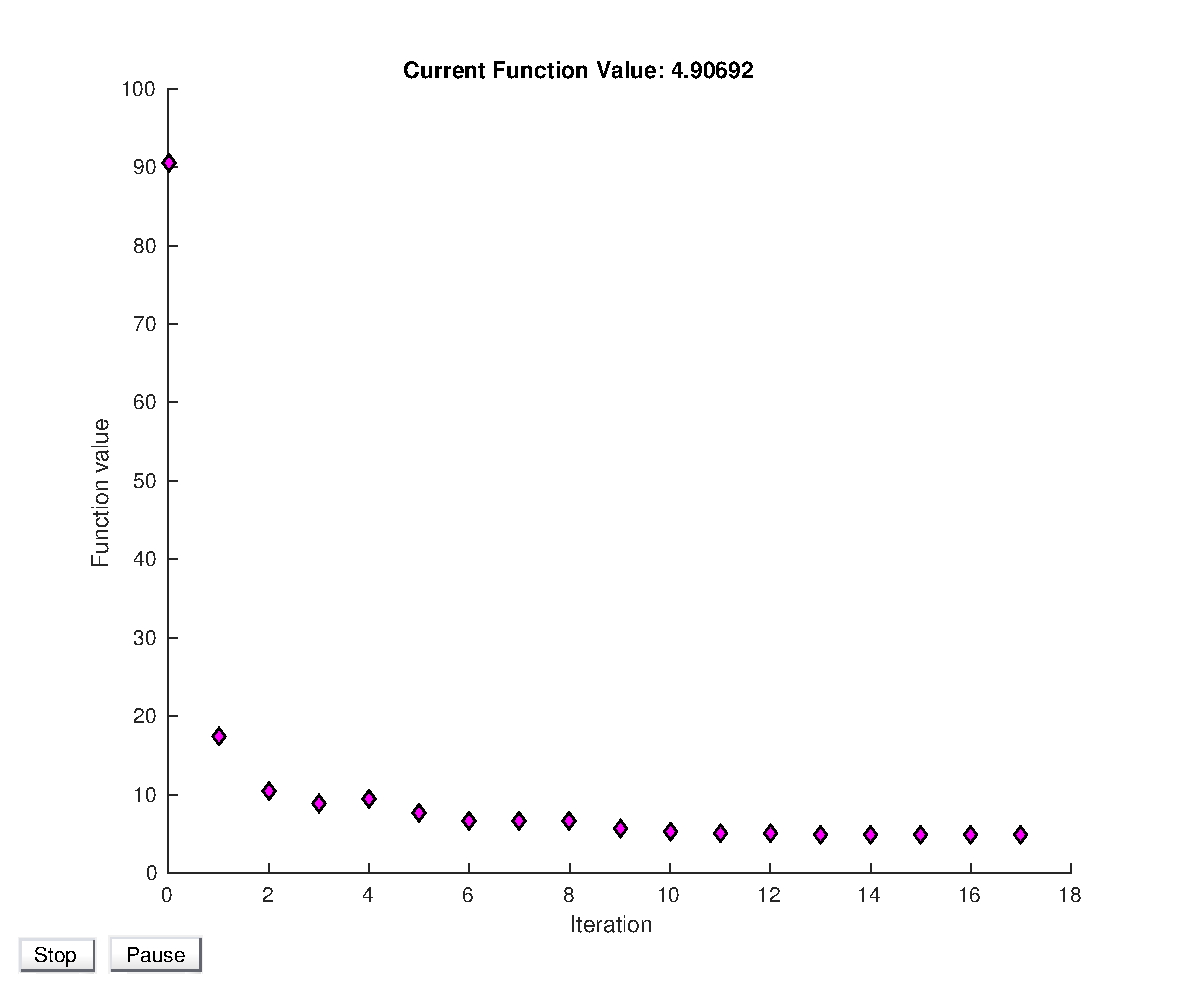
\includegraphics[width=\textwidth]{Pics/complex40opt.eps}
        
    \end{subfigure}
\end{figure}


\subsection{Source Code}
\lstinputlisting[caption=UAV Optimization Example, label=uavex]{Code/Optimisation.m}
\onecolumn
\lstinputlisting[basicstyle=\ttfamily, caption=UAV Class, label=uavclass]{Code/UAV.m}








































\end{document}